\section[Follow the truth table]{Just follow the truth table!}

% what allows us to design CPUs is that we have a good theory of what the world is like. This allows us to construct things in our mind before testing whether those abstractions worked.
% This is the basis of all modern technology.

\frame{
	\begin{center}
		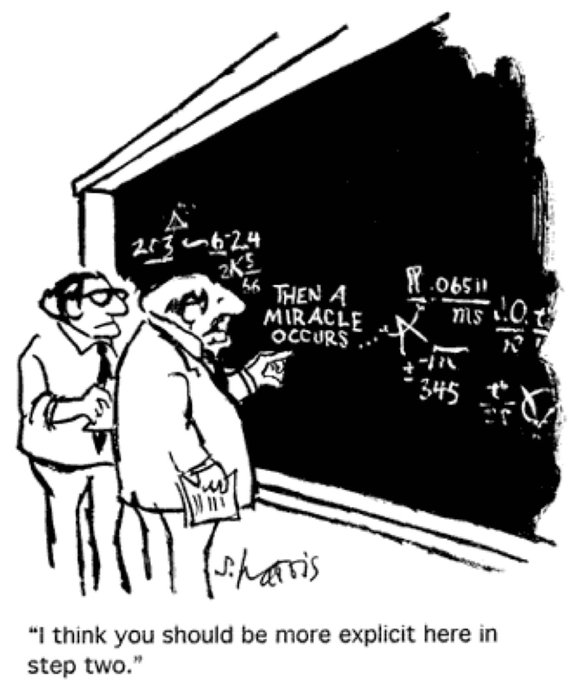
\includegraphics[height=0.76\textheight]{miracle.jpg}
	\end{center}
	\cite{thenamiracleoccurs}
}

\note{
	\begin{itemize}
		\item Before we can develop really good software, we need to demystify the computer.
		\item For some people computers are entirely like magic. You put something in -- then, magic happens -- 
			and you get something out
		\item Like there's a magic elf inside that solves these problems for you. Even for programmers.
		\item For some, like me, they're not \textit{entirely} magic anymore. I'm far from knowing
			all the details, but I think I got the gist of it right, and so I want to explain to you
			what a computer is, in philosophical terms, without the assumption of magic.
	\end{itemize}
}


\frame{
	\begin{itemize}
		\item I assume we have relays and switches.
		\item A switch interrupts a flowing current when it's in it's OFF position
		\item A relay has two inputs, a general-power input and a control input.
		\item It's function is to output power, once the control switch is on and not
			output power when it's off.
	\end{itemize}
}

\begin{frame}
	\begin{center}
		%\movie[width=10.35cm,height=5.811cm,poster,loop]{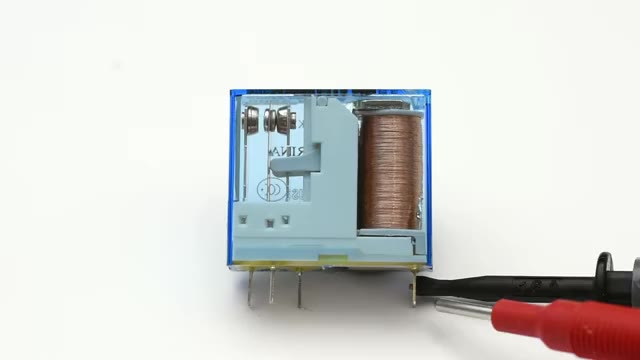
\includegraphics[width=10.35cm,height=5.811cm]{firstframerelais.jpg}}{relais.mp4}

		\href{run:relais.mp4?autostart&loop}{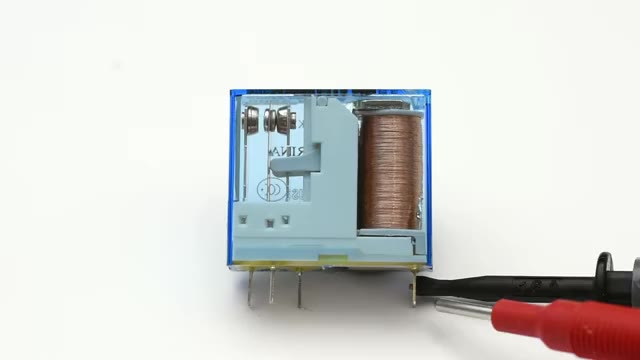
\includegraphics[height=0.7\textheight]{firstframerelais.jpg}}
	\end{center}
	\citetitle{wikirelais}
\end{frame}


\frame{
	\begin{center}
		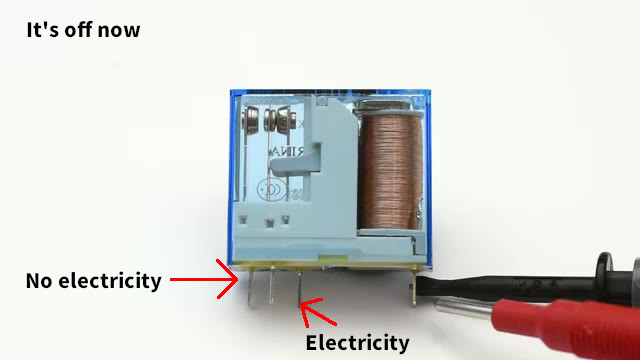
\includegraphics[width=0.7\textwidth]{not_relais.jpg}
	\end{center}
}

\frame{
	\begin{center}
		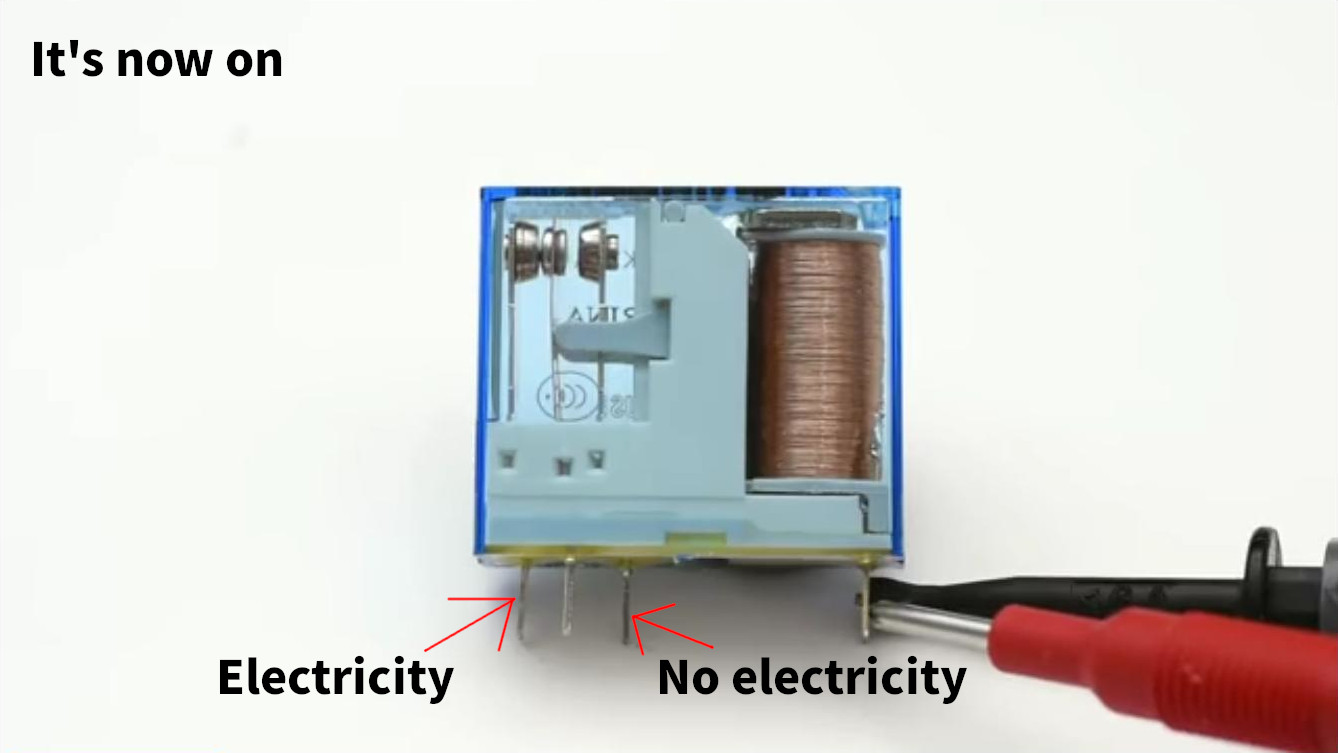
\includegraphics[width=0.7\textwidth]{relais_on.jpg}
	\end{center}
}

\frame{
	\begin{itemize}
		\item A function has an input-vector and an output-vector.
		\item $z = f\left(\begin{bmatrix}
				x\\
				y
		\end{bmatrix}\right) = \begin{bmatrix}
			x^2 \\
			x + y\\
			y^2
		\end{bmatrix}$ for example
	\item Or \texttt{AND}: $z = f\left(\begin{bmatrix}
			x\\
			y
	\end{bmatrix}\right) = \begin{bmatrix}
		x \wedge y
	\end{bmatrix}$
	\end{itemize}
}

\note{
	\begin{itemize}
		\item For this, let's very quickly turn to formal logic and math. I assume you have a basic idea of what that is.
		\item Let's imagine, our input $x$ and $y$ can only be one or zero, nothing else and keep the coventions for operations
			(this called a \textit{ring of integers of modulo n})
		\item We want to define one of the most basic parts of a CPU, an ALU (algorithmic-logical unit).
		\item There are many more parts to a CPU, like control flow units, but we are going to ignore those.
		\item Let's define an \texttt{AND}.
	\end{itemize}
}

\frame{
	Let's look at the truth-table of \texttt{AND}.

	\begin{table}[]
		\begin{tabular}{l|l|l}
			$a$ & $b$ & $a \mathrm{\ AND\ } b$ \\ \hline
			0 & 0 & 0       \\
			0 & 1 & 0       \\
			1 & 0 & 0       \\
			1 & 1 & 1
		\end{tabular}
	\end{table}
}


\note{
	\begin{itemize}
		\item See it? It's only true when both $a$ and $b$ are true.
		\item Let's construct this.
	\end{itemize}
}

\frame{
	{\Huge $a$ \texttt{AND} $b$:}
	\begin{center}
		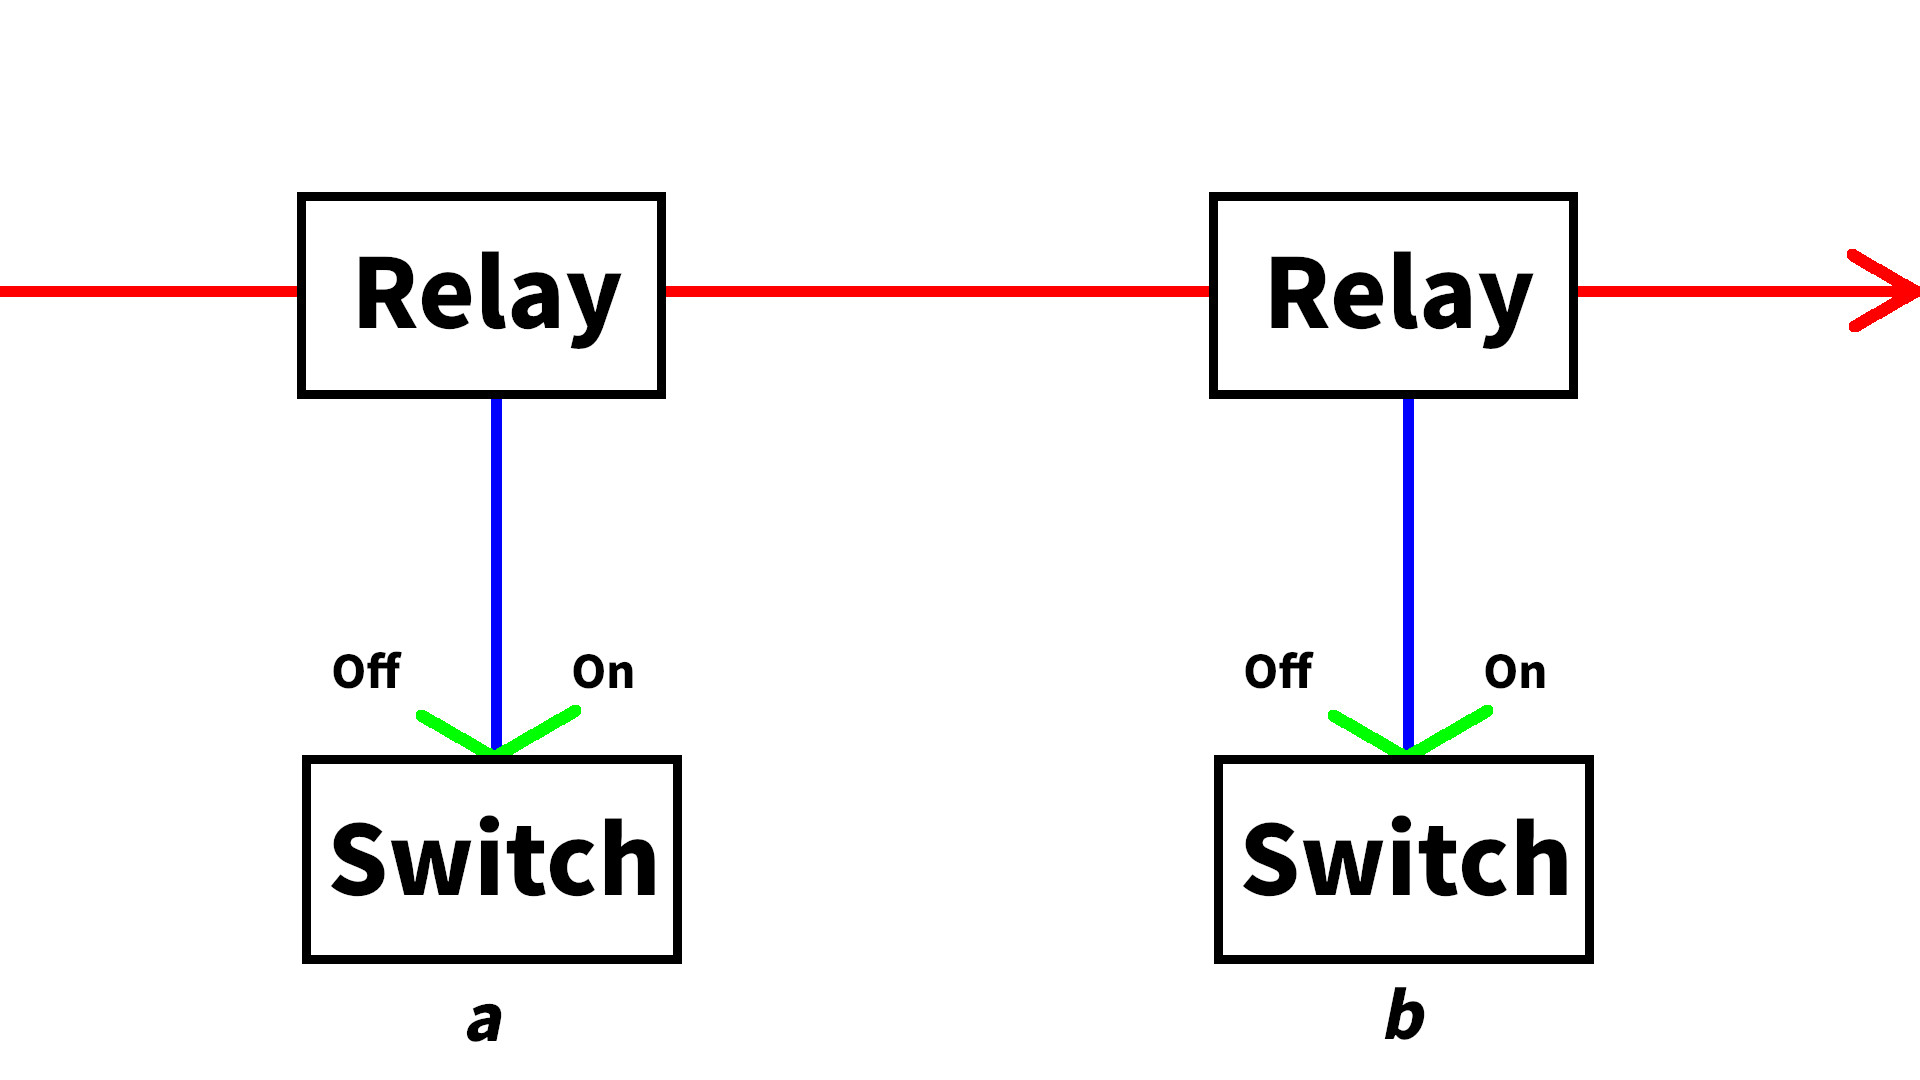
\includegraphics[width=0.8\textwidth]{and.jpg}
	\end{center}
}


\note{
	\begin{itemize}
		\item See? This can only be ON once both the $a$-switch and the $b$-switch are on. Otherwise, nothing comes out of this circuit.
		\item Now, this is not only a circuit, but the starting moment of modern computing.
		\item The idea is to use the natural laws of the universe (like the laws of electricity or flowing water) in such a way that they can 
			represent a truth table
		\item All modern computing is based on the creation of analogies of internal mental structures in the outside-world
		\item (I personally believe that this is because logic itself is an analogy of the world, so that we have the ability to manipulate
			things in our mind, and this ability is what differentiates humans from all other animals. Computers allow us to outsource
			the simplest form of thinking to a machine.)
		\item Only in the moment of inputting something and the moment of reading the outputs, the computer is really `calculating'. Inbetween,
			it's just doing physics.
	\end{itemize}
}



\frame{
	\begin{center}
		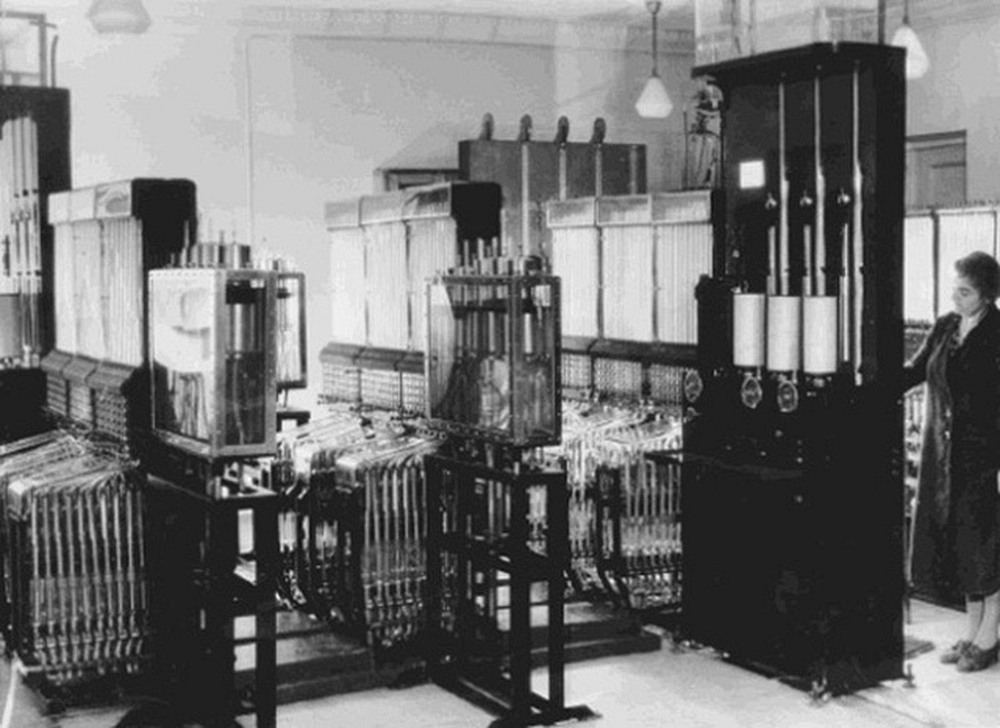
\includegraphics[width=0.6\textwidth]{integrator.jpg}
	\end{center}

	\cite{integratorbild}
}


\note{
	\begin{itemize}
		\item This analogy-idea of a computer can be transferred to quasi infinite many different ways.
		\item You can build computers with relays or with transistors. For the logic, it doesn't matter.
		\item You can even build computers that run on water, because you could choose water instead of electricity.
		\item This has been done btw.
		\item You even could build this from vacuum chambers and vacuum valves. With that idea, either there is a 
			good vacuum (1) or there's not (0). You can literally, in principle, compute anything computable
			with \textit{nothing}. You could run Linux on something that is the most \textit{nothing at all}
			we can achieve physically, if time and money were really no concern.
	\end{itemize}
}

\frame{
	Now let's define \texttt{OR} via it's truth table.

	\begin{table}[]
		\begin{tabular}{l|l|l}
			$a$ & $b$ & $a \mathrm{\ OR\ } b$ \\ \hline
			0 & 0 & 0       \\
			0 & 1 & 1       \\
			1 & 0 & 1       \\
			1 & 1 & 1
		\end{tabular}
	\end{table}
}

\frame{
	{\Huge $a$ \texttt{OR} $b$:}
	\begin{center}
		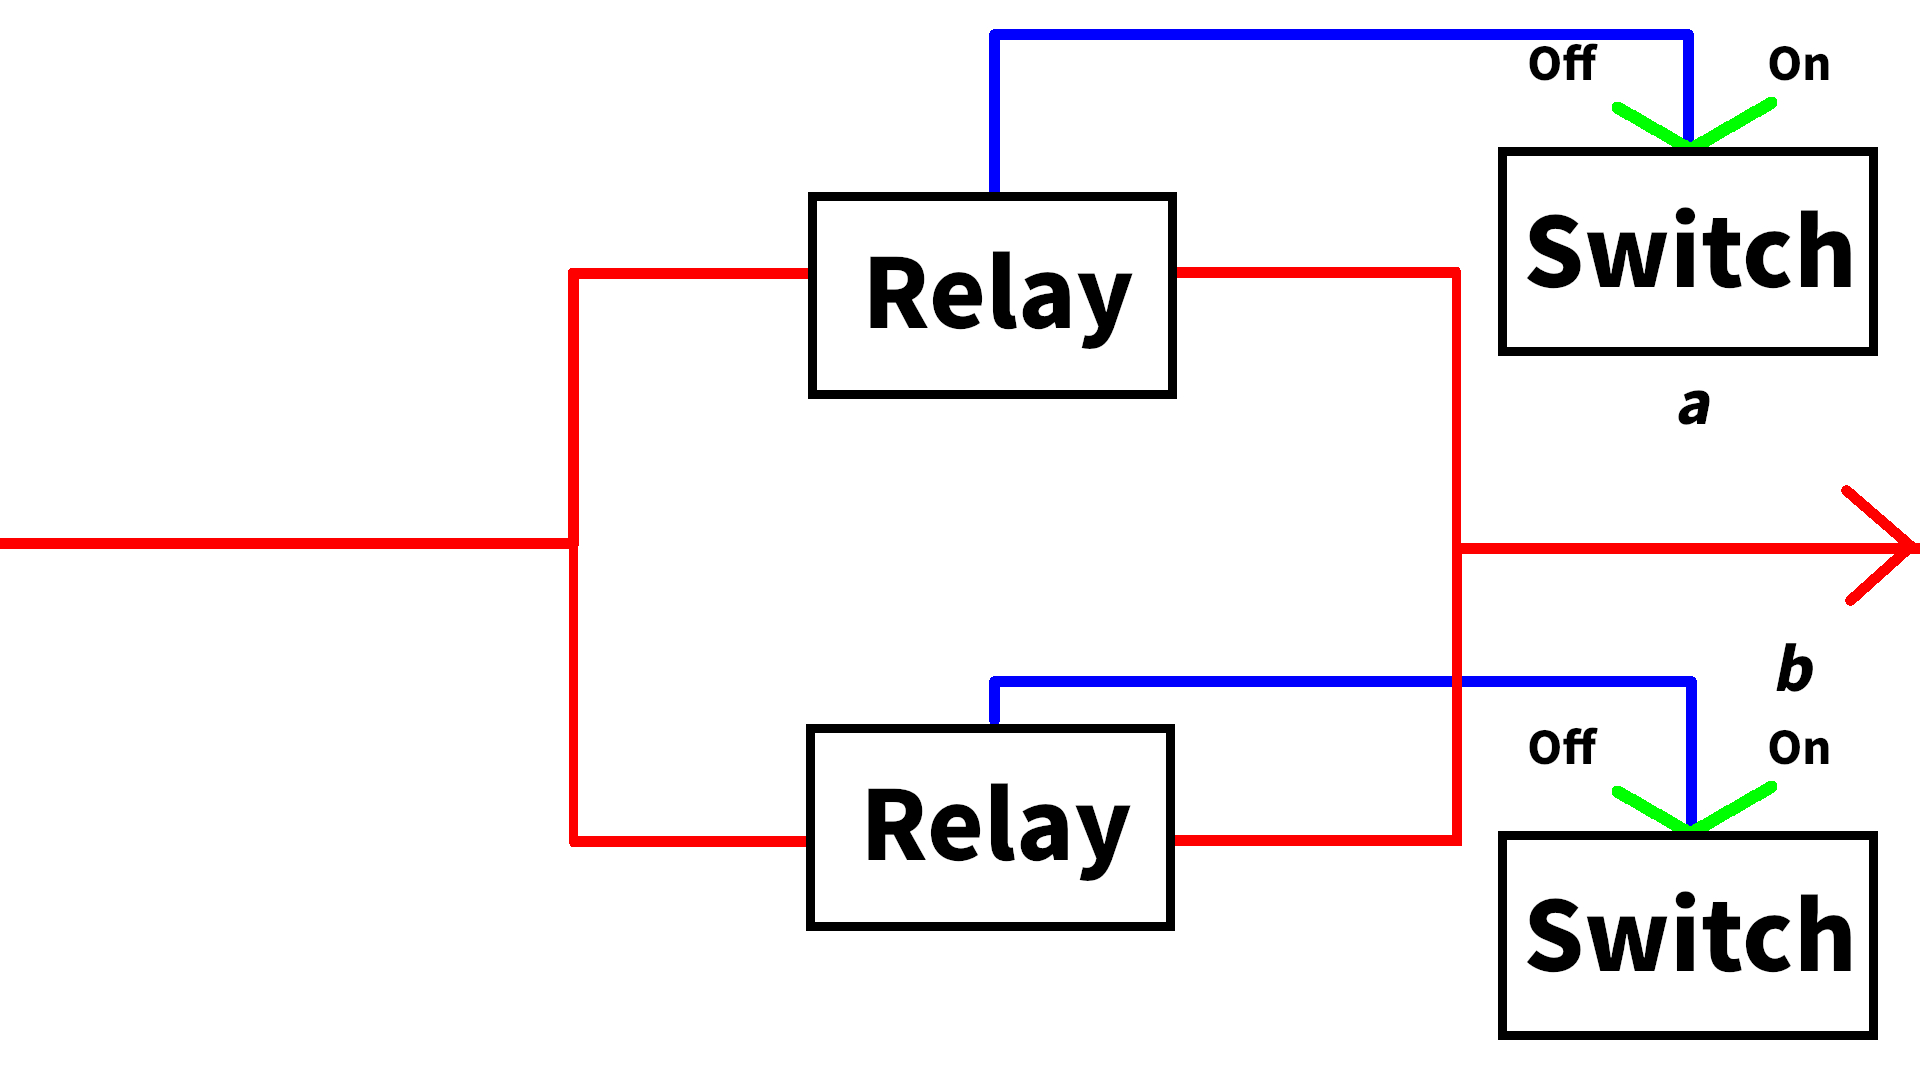
\includegraphics[width=0.8\textwidth]{or.jpg}
	\end{center}
}

\note{
	\begin{itemize}
		\item This is a logical OR. It is true when at least one input is true.
		\item At the end, there must be electricity (or water, or vacuum) if one or both switches are on.
	\end{itemize}
}

\frame{
	\begin{itemize}
		\item One last basic definition, but this one is very simple. Let's look at the truth table from \texttt{NOT}.
	\end{itemize}

	\begin{table}[]
		\begin{tabular}{l|l}
			$a$ & $\mathrm{NOT\ } a$ \\ \hline
			0 & 1      \\
			1 & 0
		\end{tabular}
	\end{table}

	\begin{itemize}
		\item This can easily be achieved by connecting the cable to the rightmost pin, so that there is no current flowing
			when the switch is on.
	\end{itemize}
}

\frame{
	{\Huge $\texttt{NOT\ } a$:}
	\begin{center}
		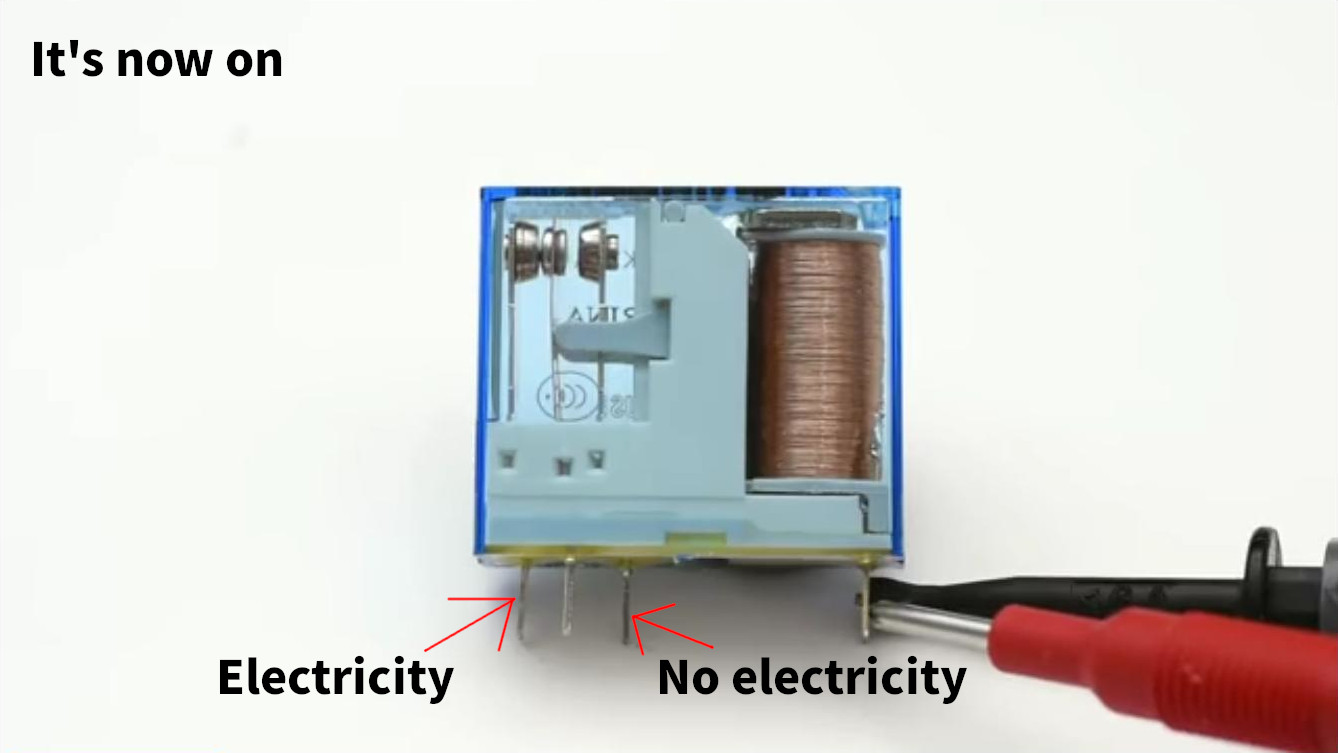
\includegraphics[width=0.7\textwidth]{relais_on.jpg}
	\end{center}
}

\note{
	\begin{itemize}
		\item See the three pins on the left? The middle one connects to the mains, and the left one is normally closed, and the right one is normally open.
		\item You can use the right one that is normally open as \texttt{NOT}. It only closes once the switch is in the on-position.
	\end{itemize}
}

\frame{
	\begin{itemize}
		\item Let's define \texttt{XOR}.
	\end{itemize}
}
\note{
	\begin{itemize}
		\item I hope you now see the connection between truth tables and the hardware and could construct something like this.
		\item Let us now go on even further a bit, but with equations only.
		\item Let's define \texttt{XOR}.
	\end{itemize}
}

\frame{
	\begin{table}[]
		\begin{tabular}{l|l|l}
			$a$ & $b$ & $a \mathrm{\ XOR\ } b$ \\ \hline
			0   & 0   & 0                  \\
			0   & 1   & 1                  \\
			1   & 0   & 1                  \\
			1   & 1   & 0
		\end{tabular}
	\end{table}

	\begin{itemize}
		\item You can see: \textit{it's only on when either (a is on and b off) or (a is off and b is on)}.
		\item $\left(a \mathrm{\ AND\ NOT\ } b\right) or \left(\mathrm{NOT\ } a \mathrm{\ AND\ } b\right)$
		\item We have all of these. So we do not need new hardware part designs, but only to merge already existing
			modules (\texttt{AND}, \texttt{NOT} and \texttt{OR}).
	\end{itemize}
}


\note{
	\begin{itemize}
		\item Imagine putting a lamp at the end of this.
		\item If we leave `is on', it is directly the logical notation equivalent to XOR. And this is all we need.
		\item From this, you can construct \texttt{XOR}. You now saw how each of them is realized. You've seen
			\texttt{AND}, \texttt{OR} and \texttt{NOT}.
	\end{itemize}
}

\frame{
	\begin{itemize}
		\item You can also now construct \texttt{NAND}, the negated \texttt{AND}:
	\end{itemize}
	\begin{table}[]
		\begin{tabular}{l|l|l}
			$a$ & $b$ & $a \mathrm{\ NAND\ } b$ \\ \hline
			0   & 0   & 1                 \\
			0   & 1   & 1                 \\
			1   & 0   & 1                 \\
			1   & 1   & 0
		\end{tabular}
	\end{table}
}

\frame{
	\begin{itemize}
		\item Or \texttt{NOR}, the negated \texttt{OR}:
	\end{itemize}
	\begin{table}[]
		\begin{tabular}{l|l|l}
			$a$ & $b$ & $a \mathrm{\ NOR\ } b$ \\ \hline
			0   & 0   & 1                 \\
			0   & 1   & 0                 \\
			1   & 0   & 0                 \\
			1   & 1   & 0
		\end{tabular}
	\end{table}
}


\frame{
	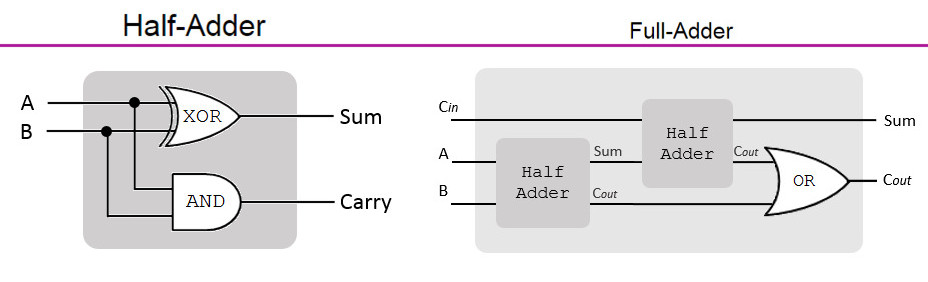
\includegraphics[width=\textwidth]{halfadderfulladder.jpg}
	\cite{halfadderfulladder}
}
\note{
	\begin{itemize}
		\item From \texttt{AND}s, \texttt{OR}s, \texttt{NOT}s and \texttt{XOR}s, you can build adders, subtractors, 
			multipliers and so on. Each one cares less about the direct implementation of the lower layers. It gets
			more abstract.
		\item The final layer should be the most abstract: the user-level of the program. You have good software when 
			the user does not need to worry about \textit{any} of the underlying details.
		\item And you can get more and more abstract (that is, removed from concrete hardware).
			Once you have a module you know acts like an Adder,
			just label it Adder and don't care about the exact underlying structure. Do this in all of your programs,
			so that the end-user does not need to care about implementation details in any way.
	\end{itemize}
}


\frame{
	\begin{center}
		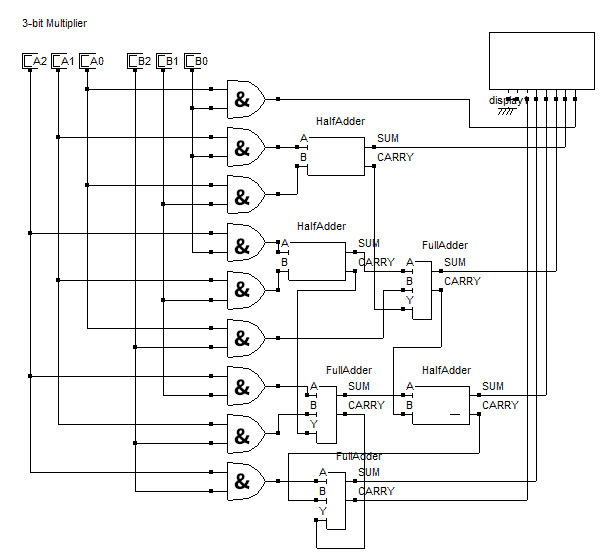
\includegraphics[width=0.5\textwidth]{mult.jpg}

		\cite{multiplier}
	\end{center}
}

\frame{
	\begin{itemize}
		\item For a general outline, we just need the \texttt{JMP}-instruction now.
		\item \texttt{JMP} is able to `jump' from one part of the code to another, similiar to \texttt{goto} in the basic idea
		\item Most CPUs define multiple jump-functions like \texttt{JE} (jump if equal), \texttt{JNE} (jump if not equal),
			\texttt{JG} (jump if greater), \dots
		\item With jump-instructions, you can do branches, very similiar to this Pseudo-Code:
	\end{itemize}
}

\begin{frame}[fragile]
\begin{lstlisting}[language=C]
if(a == 5) { // jump if a == 5
	goto A_EQUAL_FIVE;
} else { // jump if a != 5
	goto A_NOT_EQUAL_FIVE;
}
return;
A_EQUAL_FIVE:
printf("a==5");
return;
A_NOT_EQUAL_FIVE:
printf("a!=5");
return;
\end{lstlisting}
\end{frame}


\frame{
	\begin{itemize}
		\item When you have adders, you can build multipliers of them (as, with the integers at least, multiplication is just repeated addition).
		\item When you have multipliers and branch-statements like \texttt{JE}, you can use them to create a faculty function like that:
			$$
				n! = \begin{cases}
					1 & \mathrm{if}\ n == 1 \\
					(n-1)! & \mathrm{else}
				\end{cases}
			$$
	\end{itemize}
}

\frame{
	Assuming you also have a divison circuit, which we will also skip here, you can then build:

	$$\sin(x) = \sum_{n=0}^\infty (-1)^n\frac{x^{2n}}{(2n)!} = \frac{x^0}{0!}-\frac{x^2}{2!}+\frac{x^4}{4!}\mp\dotsb$$

	And with that work on even more and more complex structures, not caring about the detail-implementation anymore.
}
\note{
	\begin{itemize}
		\item This is what libraries do for you.
		\item When you do $\sin(x)$ in C, it gets breaken down to the taylor series shown
		\item This then gets broken down to a lot of \texttt{AND}s, \texttt{XOR}s and \texttt{NOT}s.
		\item Programs as I think most programmers understand them are usually only `glueing together' libraries,
			things that abstract away from the hardware that you don't have to think about the logical implementation.
		\item When it's there, the $\sin$ can be used to calculate all kinds of things. Every 3D-game you ever played used these
			as libraries for the graphics for example. And the developer did not need to re-invent the wheel.
	\end{itemize}
}


%\frame{% TODO
%So the reason you can do this
%	% https://youtu.be/erc1Qrjl1oY
%	is the development of math of the last 2000 years,
%	and of logic for the last 2500 years
%	and finally because of this guy:
%	aristotle,
%	who first had the idea of formalizing logic.
%}


\frame{
	\begin{center}
		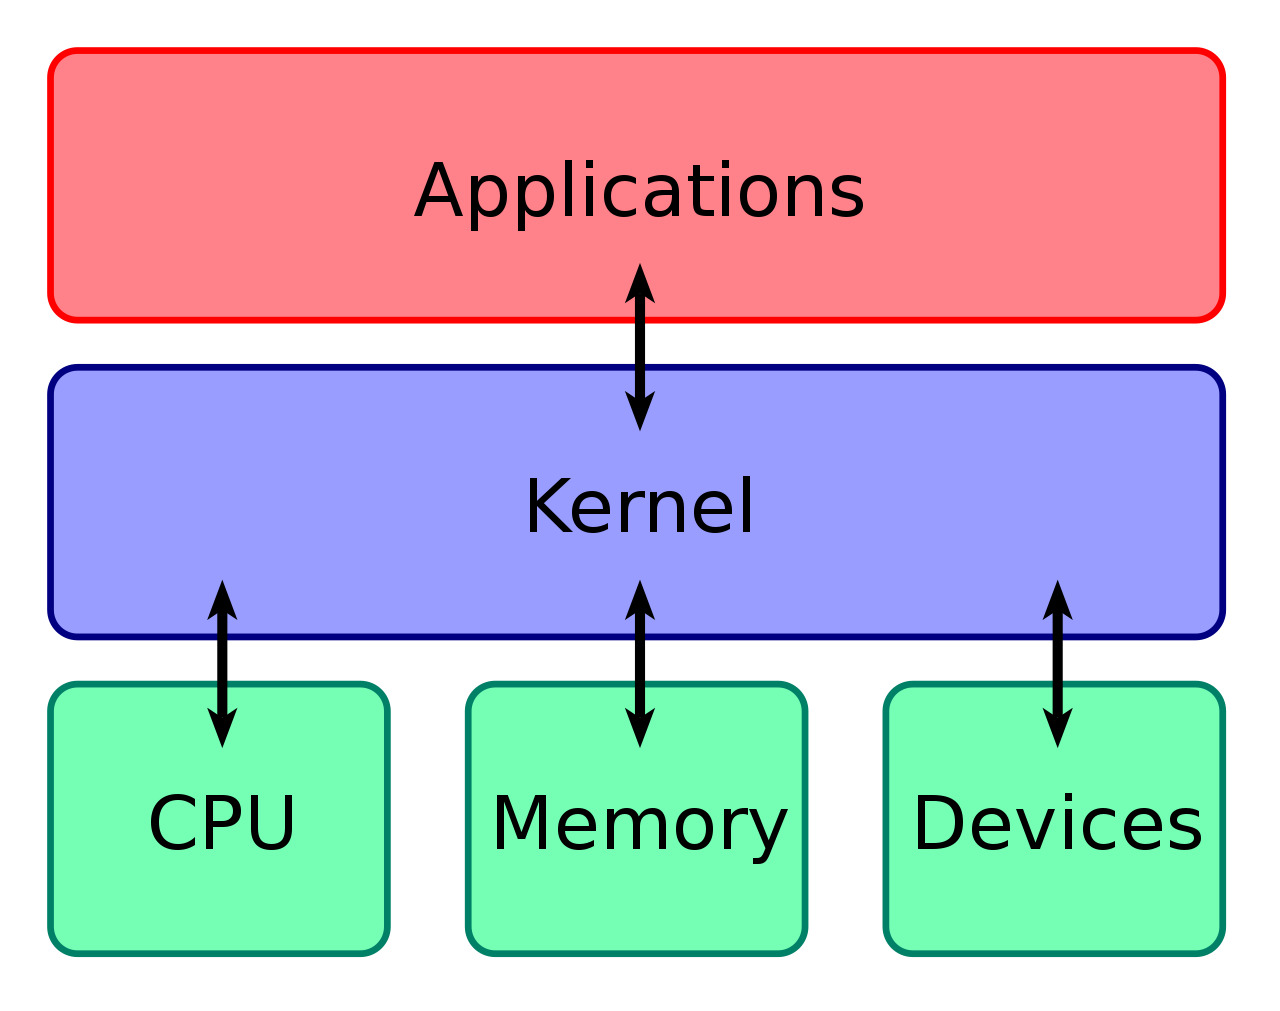
\includegraphics[width=0.8\textwidth,height=0.8\textheight,keepaspectratio]{kernel.jpg}
	\end{center}
	\cite{wikikernel}
}
\note{
	\begin{itemize}
		\item The quest for more and more abstract ways of programming leads us to operating systems.
		\item An OS is a piece of software that abstracts away the concrete hardware.
		\item The \textit{kernel} is what communicates with the hardware, and your software communicates
			with the kernel.
		\item The kernel allows you to execute certain commands, abstracted away from the real hardware,
			so you don't need to care about a specific implementation of \texttt{AND}s and \texttt{XOR}s, but only
			about doing basic level mathematics for example.
	\end{itemize}
}

\frame{
	\begin{center}
		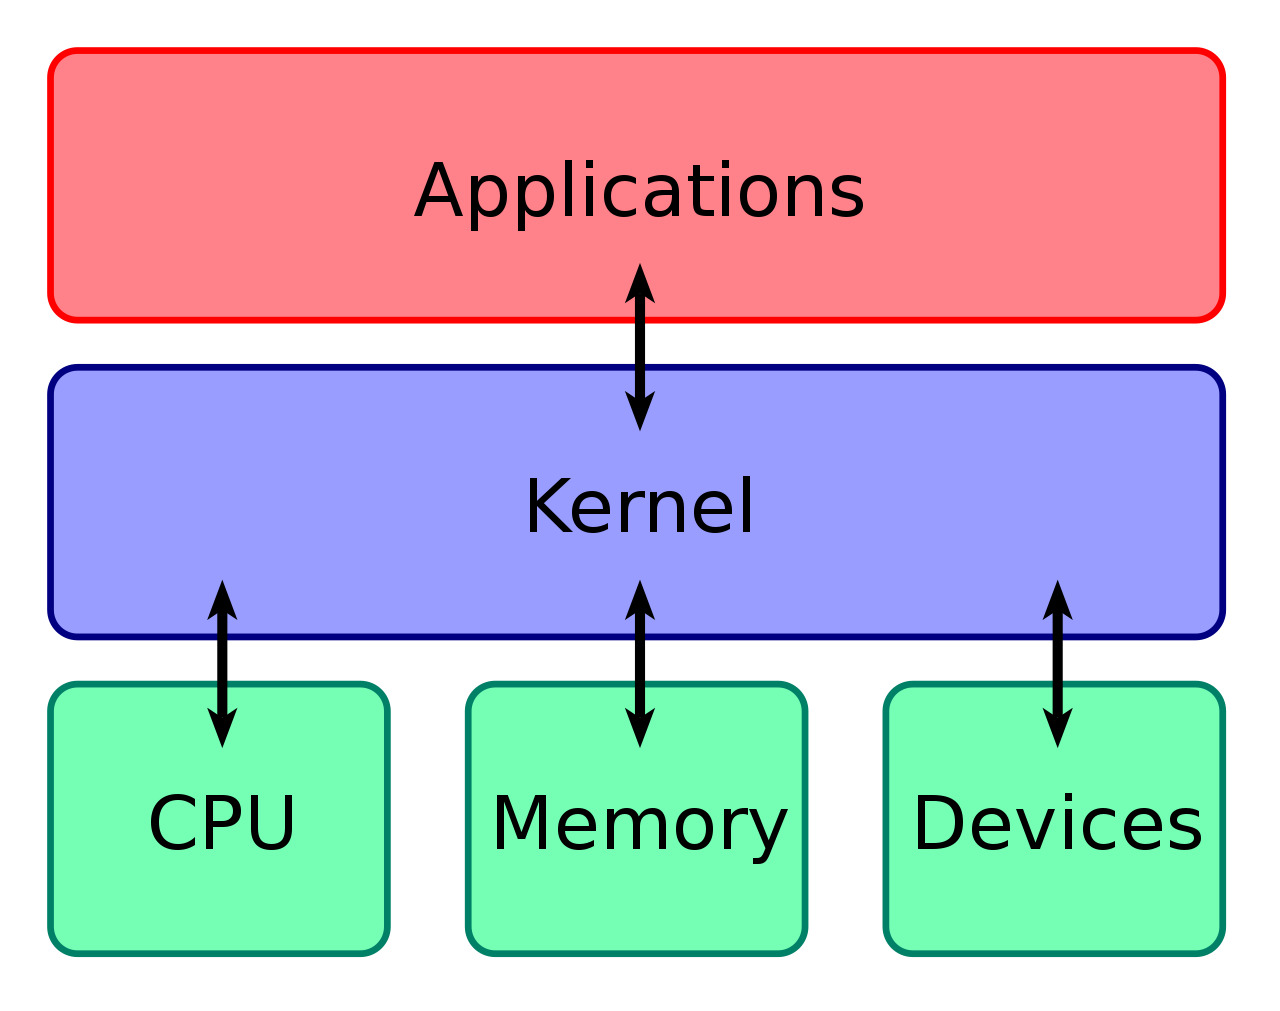
\includegraphics[width=0.8\textwidth,height=0.8\textheight,keepaspectratio]{kernel.jpg}
	\end{center}
	\cite{wikikernel}
}
\note{
	\begin{itemize}
		\item Having a kernel has the advantage that you don't need to care about communication with the hardware, only
			with the kernel. The kernel communicates with the specific hardware for you.
		\item The OS also allows you to communicate with other hardware, like printers, over a generalized
			interface. The OS needs a driver (a piece of software that tells the kernel how to use certain pieces
			of hardware), and then you can use the OS's features with that hardware, without caring about
			the intricacies of the printer.
	\end{itemize}
}


\frame{
	\begin{itemize}
		\item This is also what higher-level-languages do.
		\item The idea of a high level programming language is that, for programming them, you don't need to care about implementation details.
		\item They abstract things away from you. And I guess it's easier to find a python developer than a assembly-expert because of exactly that.
		\item Coding in assembly is much harder because you need the ability for higher mental workload.
		\item Not only the problem you really care to solve, but also additional problems (implementation details)
	\end{itemize}
}

\note{
	\begin{itemize}
		\item Please always remember that all of this would not have been possible without philosophers like
			Aristotle, who first had the idea of formalizing logic, or George Bool, who first researched
			`boolean arithmetic', or Descartes, who first researched function theory.
		\item Most of those discoveries were, at their time, regarded as `useless'
		\item See `\citetitle{hardy1967mathematician}' by G.~H.~Hardy (1940), in which he claims that number theory,
			is one of the most beautiful mathematical areas, despite it not \frqq\textit{being able to be used for anything}\flqq
		\item He was right and wrong at the same time. It is the most beautiful mathematical area, but today also
			one of the most useful ones. Without developments in number theory, the internet would not have been
			possible as it is today (no cryptography would be possible without advancements in math made some houndreds or even
			thousands of years ago that, at their time, seemed useless to most people).
		\item So remember, sometimes `the most useless' things may turn out to be the most useful things to later generations.
	\end{itemize}
}


\fullpageimage{white}{vonneumann.jpg}{wikivonneumann}

\note{
	\begin{itemize}
		\item What I've skipped:
		\item My description of what a computer is is far from complete here. For it to run as you are now used to, you need memory, for example,
			and you need way more transistors than I could possibly draw. Also, you need a control unit for your CPU. And so on.
		\item But this should give you just the right gist of thinking about the central part of your computer that is usually more mystified than
			clear to most people.
		\item If you want to learn more about this, search for \textit{Von-Neumann-Architecture}. This here was just intended to demystify the
			very basics.
	\end{itemize}
}

\frame{
	\begin{itemize}
		\item What does this practically mean?
		\item You must try to \texttt{catch} any errors you can imagine. Assume everything can -- and will -- fail all
			the time in every conceivable way. And also in all ways that you did not consider.
		\item Did you, for example, know that \texttt{fork()} can fail and that, if not properly treated, has 
			disastrious consequences?\footfullcite{forkcanfail}
		\item Also assume everything that can be entered by a user is garbage. They'll add numbers in fields designated for
			letters, they enter $0$ in a field through which something is divided and they'll try to \texttt{chmod +x}
			and run any \texttt{jpeg}-file they own and run them with sudo.
	\end{itemize}
}

\frame{
	\begin{itemize}
		\item Also really make sure you trust your subcomponents. Proving every algorithm is not do-able in practice, but write
			as many unit tests as you can. And test the interaction between modules, too. Best auto-test all of the programs
			features.
		\item Write each positive and negative tests, so that you can test your error routines.
			If you find bugs, write a test that matches them first, and then fix them. Then you can test for the presence and absense
			of that bug.
		\item Monkey-Test your script. For webpages, I recommend \textit{gremlin.js}. You can run a simple piece of code and it will
			click randomly and enter anything into any field and press any key randomly, with as many workers in parallel as you wish.
			\begin{itemize}
				\item For X11 applications, you may look into \texttt{xdotool} (or \texttt{ydotool} for wayland).
			\end{itemize}
	\end{itemize}
}

\frame{
	\begin{itemize}
		\item You cannot trust anything from the outside. Don't assume a User will only use \texttt{ASCII} in his folder names, but
			assume strange \texttt{UTF-8} symbols from a russian encoded website from a buggy browser that modifies random bits. It must either
			work, if you really find no way of making it work, display an exact error message on what's wrong and what needs to be done
			about this. (When writing GUI-Applications, make it easily copyable so that it can be googled).
		\item Like in real life, you cannot stop things from going wrong. But you can stop them from going horribly wrong. You can catch most
			of the `wrongness' if you clean up after yourself properly and don't rely on other people to do your work
	\end{itemize}
}

% Suspect that everything will go wrong. Literally EVERYTHING. Check return-values. Use exceptions. Compile a debug-version of your software where every warning leads to hard crashes. Ideally, there should not be any warning left when you use your program. Then compile a version of it where warnings do not crash the program. Distribute that. But test with FATAL WARNINGS.
